%=========================================================================
% fig-tune-vector.tex
%=========================================================================

\begin{figure}[h]

  \centering
  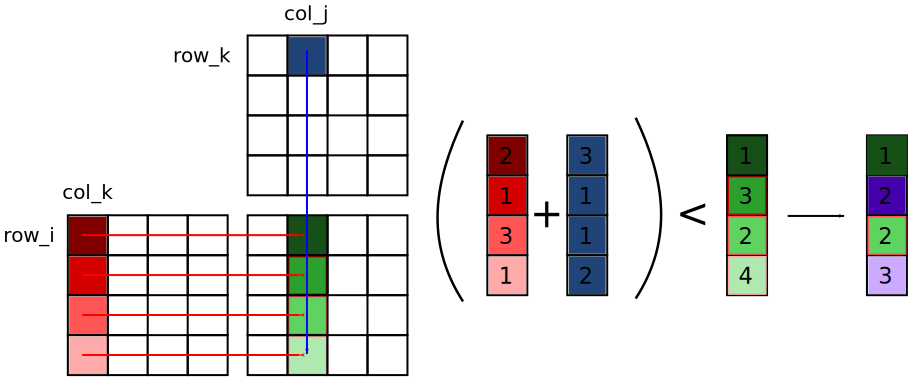
\includegraphics[width=0.9\tw]{fig-tune-vector.svg.pdf}

  \caption{\textbf{Overview of Manual Vectorization Strategy --} All
    matrices shown on the left side represent the same shortest path
    matrix. The elements of the k-th column are added to the (k,j)-th
    element and compared against the current shortest path value in the
    (i,j)-th element. An example vectorized computation with a vector
    length of 4 is shown on the right, where the final result to be
    stored only contains the elements with the shortest paths between the
    sum vector and the current vector. }

  \label{fig-tune-vector}

\end{figure}
